
\documentclass{article}

\usepackage[utf8]{inputenc}
\usepackage[russian]{babel}
\usepackage{amssymb}
\usepackage{graphicx}

\title{Определение сорта вина на основе химических исследований \\ \large \textbf{Аннотация}}

\author{Роман Логинов}
\date{\today}

\begin{document}
\maketitle

\section{Цель}

\indent\indent Целью исследования являлось построение модели для классификации сорта вина на основе показателей химических исследований, а также сравнение моделей с различными гиперпараметрами и подбор оптимальной.

\section{Выбранные модели и метрики}

\indent\indent Согласно описанию данных, всего в датасете находятся описания вин 3 сортов. Одним из методов решения задачи классификации является метод $k$ ближайших соседей.

Разбив данные на обучающую и тестовую выборки, получим, для каждого элемента из тестовой будем смотреть, к какому классу будут принадлежать его ближайшие $k$ соседей из обучающей выборки. Среди этого набора классов выберем тот, который встречается чаще всего среди этих $k$

Ближайшие соседи выбираются согласно некоторой метрике, которая является гиперпараметром модели. Приведём метрики, которые будут использованы, а также формулу для их вычисления по двум векторам из пространства $\mathbb{R}^n$

* Евклидово расстояние $\rho(x, y) = \sqrt{\sum\limits_{i = 1}^n (x_i - y_i)^2}$

* Манхэттенское расстояние $\rho(x, y) = \sum\limits_{i = 1}^n |x_i - y_i|$

* Метрика Чебышёва $\rho(x, y) = \max\limits_{i = 1}^n |x_i - y_i|$

Ещё одним гиперпараметром является количество соседей, которое просматривается. Попробуем исследовать, как изменится качество модели, если варьировать гиперпараметры.

Для оценки качества будем использовать метрику `accuracy`, которая равна доле правильных ответов на тестовой выборке. Конечной целью будет максимизация этой метрики.

Более того, для применяемой модели очень важен порядок величины различных признаков. Если признаки не отнормировать, то вклад одинаковых в процентном соотношении отклонений величины параметров в расстояние между точками будет разным.

\bigskip
Ещё одним гиперпараметром является количество соседей, которое просматривается. Попробуем исследовать, как изменится качество модели, если варьировать гиперпараметры.

Для оценки качества будем использовать метрику `accuracy`, которая равна доле правильных ответов на тестовой выборке. Конечной целью будет максимизация этой метрики.

\section{Результаты}

\begin{center}
	\makebox[\textwidth]{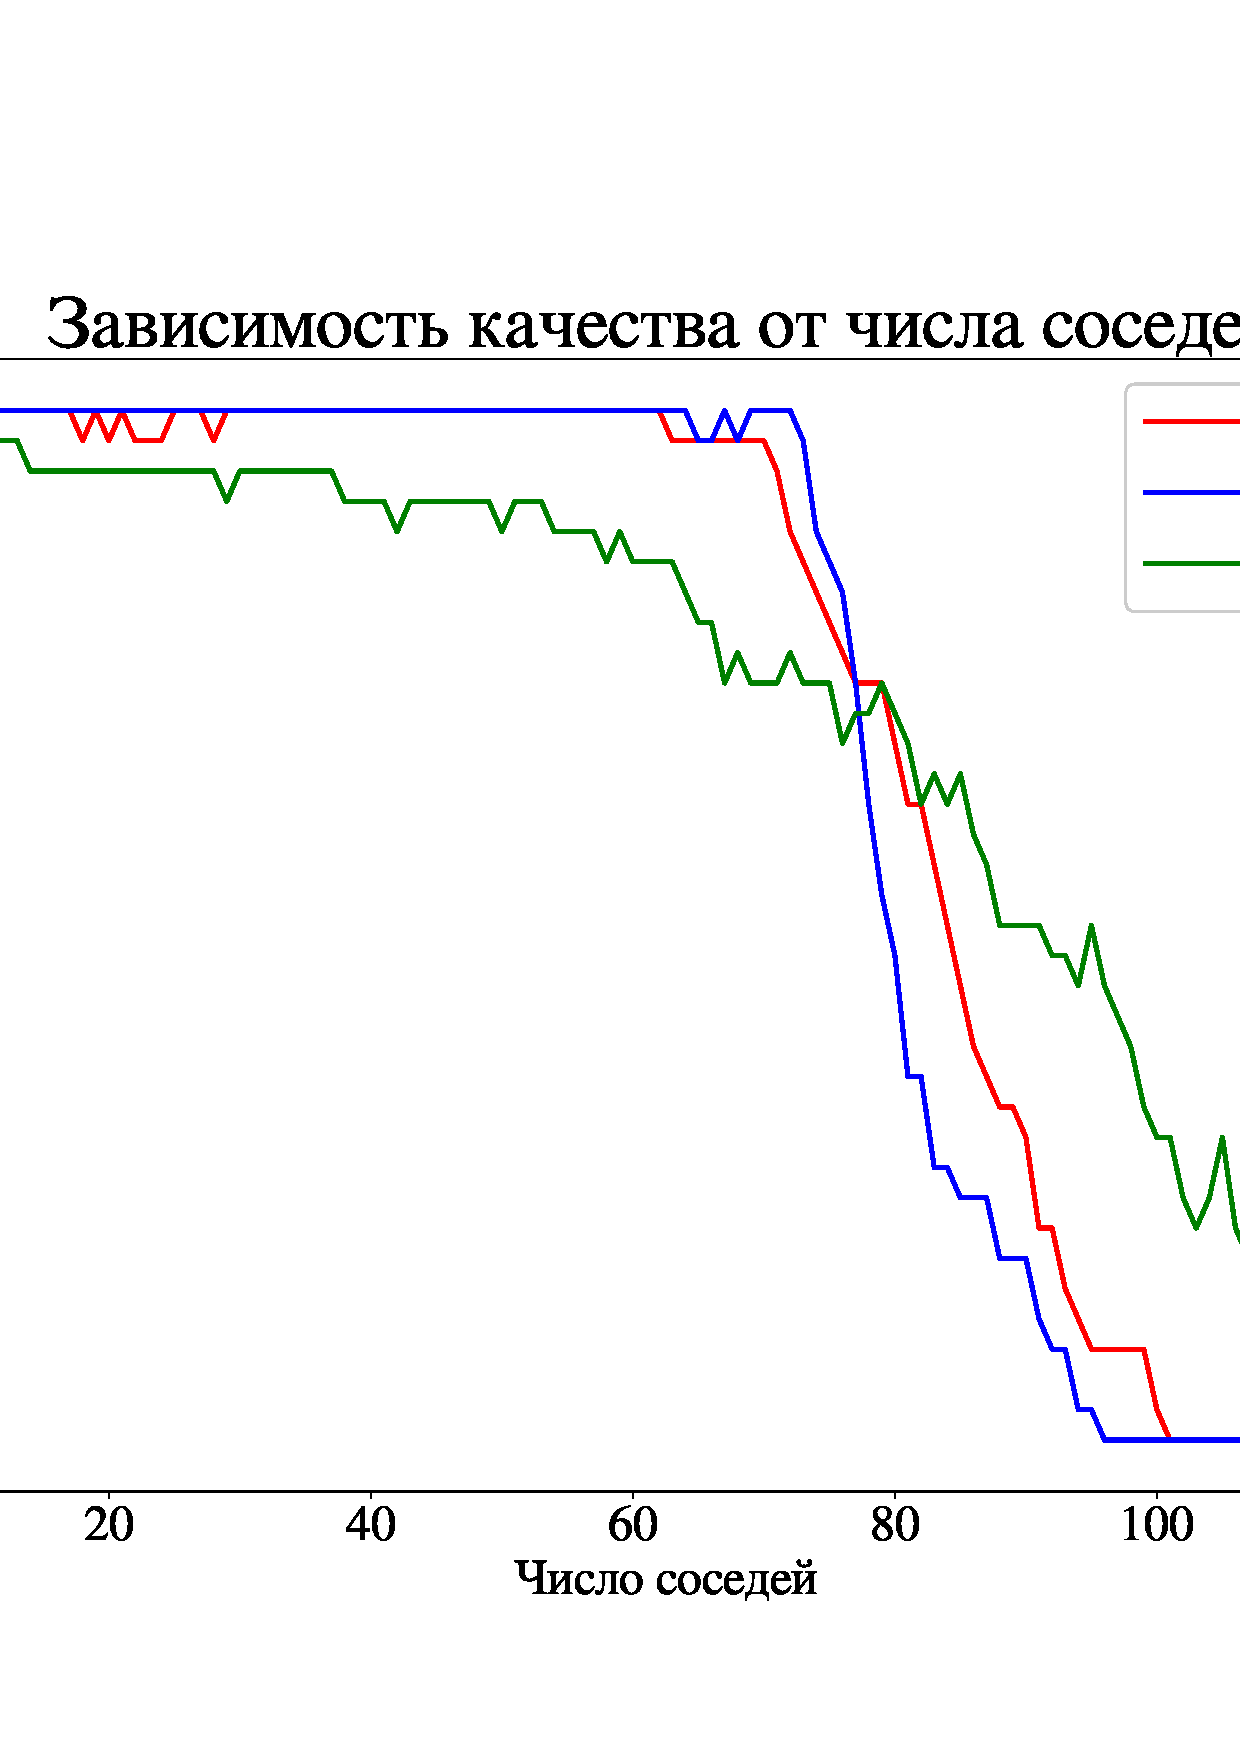
\includegraphics[width=\paperwidth]{fig.png}}
\end{center}

\section{Выводы}

Построенные модели показывают, что в целом качество модели ведёт себя одинаково при увеличении количества рассматриваемых соседей. Оптимальные значения наблюдаются при $k \leqslant 60$, затем качество начинает падать примерно линейно, и  начиная примерно с рассмотрения 100 соседей модель ведёт себя уже не лучше случайного предсказания (а точнее вырождается в константное предсказание наиболее объёмного класса)

На начальных значениях стабильнее всего и лучше ведёт себя модель, использующая манхэттенское расстояние. Использование расстояния Чебышёва оказывается хуже, однако такая модель точнее предсказывает класс при большом количестве соседей.

Видим, что лучшее значение качества достигается при использовании манхэттеновского расстояния при $k = 8$ и равно примерно $0.98$.

Интересно, что такой же эксперимент, проведённый без нормализации данных, даёт точность предсказаний не выше $0.8$ на всех трёх рассмотренных метриках

\end{document}